\section{Methods}

\subsection{Problem setting and feature representations}
We considered binary \dti{} prediction for a drug set $\mathcal{D}$ and a
protein set $\mathcal{P}$. Let $A\in\{0,1\}^{|\mathcal{D}|\times|\mathcal{P}|}$
denote the observed interaction matrix, where $A_{ij}=1$ indicates an annotated
interaction between drug $i$ and protein $j$. Each drug was represented by a
cached 1,024-bit radius-2 Morgan bit vector \cite{rogers2010ecfp}, and each protein by a cached
mean-pooled ESM-2 t30/150M embedding (640 dimensions) \cite{lin2023esm}. The drug and protein
feature encoders were distinct learnable projection networks; their parameters
were not shared.

We constructed a drug similarity matrix $S_D$ and a protein similarity matrix
$S_P$ by cosine similarity of the corresponding cached feature vectors. These
similarities were feature-derived and were not calculated from DTI labels.

\begin{figure*}[t]
\centering
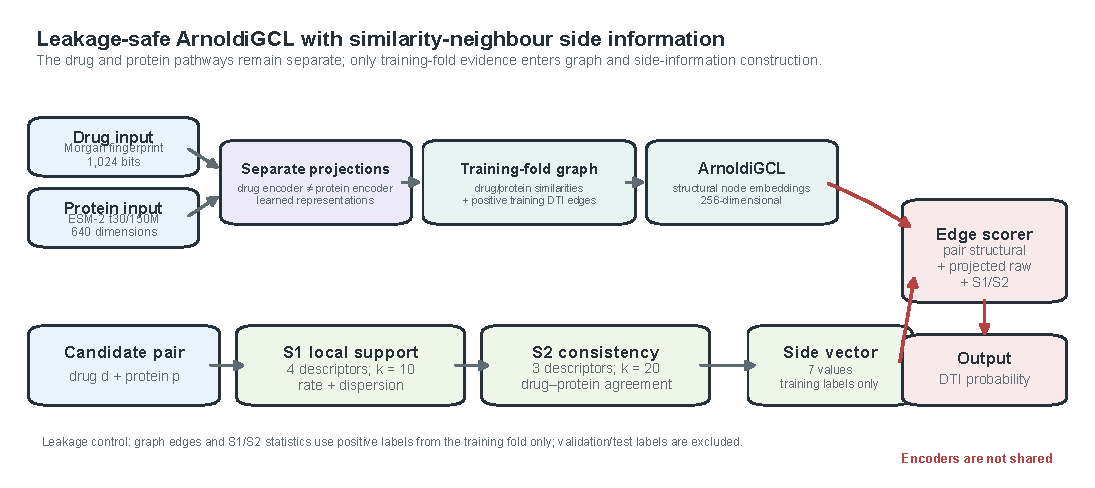
\includegraphics[width=\textwidth]{figures/figure_1_method_schematic.pdf}
\caption{Overview of the full ArnoldiGCL-S1/S2 DTI predictor. Drug Morgan
fingerprints and protein ESM-2 embeddings enter distinct learnable projection
networks; the encoder weights are not shared. A training-fold graph supplies
structural embeddings, while the S1/S2 branch derives seven candidate-pair
descriptors from feature-based neighbours and positive $A_{\mathrm{train}}$
edges only. Structural pair features, raw features and side information are
then combined by an edge scorer. Validation and test DTI labels are excluded
from graph and side-information construction.}
\label{fig:method-overview}
\end{figure*}

\subsection{Leakage-safe graph construction}
For every outer fold, the graph contained only positive DTI edges from the
training partition. Drug--drug and protein--protein similarity edges were also
restricted to entities observed in that training partition. The default graph
connected the top 10 drug neighbours and top 10 protein neighbours; all graph
edges were represented bidirectionally. The Threshold GCN baseline instead
retained within-type similarity edges whose similarity exceeded 0.3. No
validation or test DTI labels were added to a graph or side-information feature.

\subsection{ArnoldiGCL structural representation}
The projected drug and protein features were concatenated as nodes in the
training-fold graph and passed to the ArnoldiGCL encoder
\cite{coskun2025arnoldigcl}. The structural
embedding dimension was 256. The downstream edge scorer received the structural
embeddings of a candidate drug--protein pair together with the respective raw
Morgan and ESM-2 representations. The encoder was optimized for 50 epochs, and
each edge scorer was optimized for 200 epochs with Adam (learning rate
$10^{-3}$ and dropout 0.5). For encoder pretraining, the objective was binary
discrimination between the graph representation of the projected node features
and a negative view formed by a random permutation of node features. Each
update used two positive and two negative node-level logit sets, optimized with
binary cross-entropy. The drug and protein projections remained separate
throughout this objective.

\subsection{Leakage-safe S1/S2 side information}
For a candidate pair $(i,j)$, all side information was computed from the binary
matrix $A_{\mathrm{train}}$ that contains positive training DTI edges only. Let
$N_D^k(i)$ and $N_P^k(j)$ be the top-$k$ most similar training drugs and
proteins, respectively. A queried entity was excluded from its own
neighbourhood.

The S1 module used $k=10$ and produced four descriptors: the mean and standard
deviation of $A_{d,j}$ over $d\in N_D^{10}(i)$, and the mean and standard
deviation of $A_{d,p}$ over $d\in N_D^{10}(i), p\in N_P^{10}(j)$. Thus, S1
summarizes local neighbour support and its dispersion without accessing the
label of the candidate pair.

The S2 module used $k=20$ and produced three consistency descriptors: the mean
of $A_{d,j}$ over $d\in N_D^{20}(i)$, the mean of $A_{i,p}$ over
$p\in N_P^{20}(j)$, and the mean of $A_{d,p}$ over the corresponding drug and
protein neighbour cross-product. The seven S1/S2 values were passed through the
side-information branch of the edge scorer. The S1-only and S2-only ablations
zero-padded the complementary descriptors; the shuffled control permuted the
seven-dimensional side-information vectors within each partition while
preserving their marginal distribution.

\subsection{Comparators and implementation details}
The benchmark includes logistic regression and an MLP on concatenated Morgan
and ESM-2 representations, a two-layer GCN on the leak-safe $k$NN graph, a
Threshold GCN comparator, and DrugBAN
\cite{ozturk2018deepdta,nguyen2021graphdta,bai2023drugban}. All compared methods
use the same frozen positive partitions and partition-specific negative
examples. This aligns the evaluated drug--protein pairs across methods but
does not force identical input modalities: DrugBAN consumes canonical
SMILES-derived graphs and protein sequences, whereas the feature and graph
comparators use the frozen Morgan and ESM-2 representations described above.
DrugBAN is consequently reported as a matched-partition comparator in this
benchmark, not as a claim to reproduce its published benchmark scores.
For DrugBAN, deterministic SMILES-to-graph and protein integer
preprocessing was cached within a fold when an input recurred; this does not
alter the DrugBAN architecture, optimizer or emitted batch values. DrugBAN was
trained with Adam at a learning rate of $5\times10^{-5}$, batch size 64 and a
fixed 100-epoch schedule; the validation-AUC checkpoint was evaluated once on
the corresponding test partition. All DrugBAN folds used TensorFloat-32 matrix
operations on NVIDIA GeForce RTX 4080 SUPER GPUs; this execution setting was
recorded in every
result artifact and held fixed across B5 folds.
The two GCN baselines use cached sparse normalized aggregation on BindingDB to
bound peak memory. This implementation was verified against the original dense
aggregation for forward output and backward gradients, and was smoke-tested on
the full BindingDB threshold graph before running the queue.
